\documentclass[10pt,twocolumn]{article}

\usepackage[margin=0.5in]{geometry}
\usepackage{microtype}
\usepackage{amsmath,amssymb}
\usepackage{booktabs}
\usepackage{graphicx}
\usepackage{subcaption}
\captionsetup{font=footnotesize,labelfont=bf,skip=3pt}
\captionsetup[sub]{font=scriptsize,skip=1pt,labelformat=simple}
\usepackage[compact]{titlesec}
\usepackage{enumitem}
\setlist{itemsep=0pt, topsep=1pt, parsep=0pt, partopsep=0pt, leftmargin=*}
\usepackage{setspace}
\setstretch{0.92}
\usepackage{xurl}
\usepackage{hyperref}

\hypersetup{colorlinks=true, linkcolor=blue, urlcolor=blue}

\setlength{\textfloatsep}{5pt plus 2pt minus 2pt}
\setlength{\floatsep}{5pt plus 2pt minus 2pt}
\setlength{\intextsep}{5pt plus 2pt minus 2pt}
\setlength{\abovecaptionskip}{1pt}
\setlength{\belowcaptionskip}{0pt}
\setlength{\columnsep}{0.22in}

\title{\vspace{-1.5em}Acne Detection and Cross-Domain Classification --- Report\vspace{-0.5em}}
\author{}
\date{}

\begin{document}
\twocolumn[\maketitle\vspace{-1.2\baselineskip}]

\section{Overview}

This project tackles two connected problems on dermatology imagery: (1) detecting individual acne lesions in ACNE04 with bounding-box object detection, and (2) transferring an acne classifier trained on ACNE04 patches to DermNet, a clinical skin-condition dataset with a substantial domain gap. Part~1 measures localization quality on a single dataset; Part~2 measures how well learned acne features generalize across imaging conditions, framing, and label distributions.

\section{Evaluation metrics}

{\small For detection: $\mathrm{IoU}=|B_{\text{pred}}\cap B_{\text{gt}}|/|B_{\text{pred}}\cup B_{\text{gt}}|$, $\mathrm{Precision}=TP/(TP+FP)$, $\mathrm{Recall}=TP/(TP+FN)$; for DermNet: $F_1=2PR/(P+R)$. I report \textbf{mAP} (COCO-style), precision/recall, and mean matched IoU@0.5 for detection; \textbf{Accuracy}, \textbf{F1}, and \textbf{AUROC} for classification.}

\section{Part 1: Object Detection on ACNE04}

\subsection{Models}

I trained two detectors spanning classic vs.\ modern: \textbf{Faster R-CNN} (Ren et al., 2015) --- two-stage, ResNet-50 FPN, COCO-pretrained --- and \textbf{YOLOv5s} (Ultralytics) --- single-stage YOLO lineage. YOLOv5 was chosen over heavier detectors (e.g.\ DINO-DETR) for efficiency and strong community baselines on small objects. The Roboflow YOLO head follows the export's class list; Faster R-CNN uses a two-class COCO head (background, acne). For matched IoU and the greedy P/R summary, predictions are treated as one lesion class so both detectors are compared on the same boxes.

\subsection{Data, training, evaluation}

ACNE04 (Roboflow): YOLO + COCO exports for fair splits. Patched \texttt{data.yaml} with absolute paths. \textbf{YOLOv5:} 50 epochs, 640px, batch 16, \texttt{yolov5s.pt}. \textbf{Faster R-CNN:} 10 epochs, SGD lr $0.005$, momentum $0.9$, wd $5{\times}10^{-4}$, batch 4, two classes. Faster R-CNN mAP and greedy Precision/Recall/mean matched IoU@0.5 are on the \textbf{COCO test} split (\path{torchmetrics.MeanAveragePrecision}, conf ${>}0.25$, IoU $\geq 0.5$). YOLO mAP@0.5, mAP@0.5:0.95, Precision, and Recall are the \textbf{last-epoch validation} metrics from Ultralytics \texttt{results.csv} (YOLO's val split in \texttt{data.yaml}), while YOLO mean matched IoU@0.5 is recomputed on the \textbf{same COCO test images} as Faster R-CNN via \texttt{torch.hub} for a fair localization comparison.

\subsection{Visualization}

Figure~\ref{fig:det-both} shows six test images per detector. YOLOv5 shows the export's class names where present; Faster R-CNN shows red boxes with confidences mostly 0.6--0.95 (higher test recall in Table~\ref{tab:det}); YOLOv5 achieves slightly higher mean matched IoU@0.5 on the shared COCO test pass.

\begin{figure*}[t]
\centering
\begin{subfigure}[t]{0.49\textwidth}
\centering
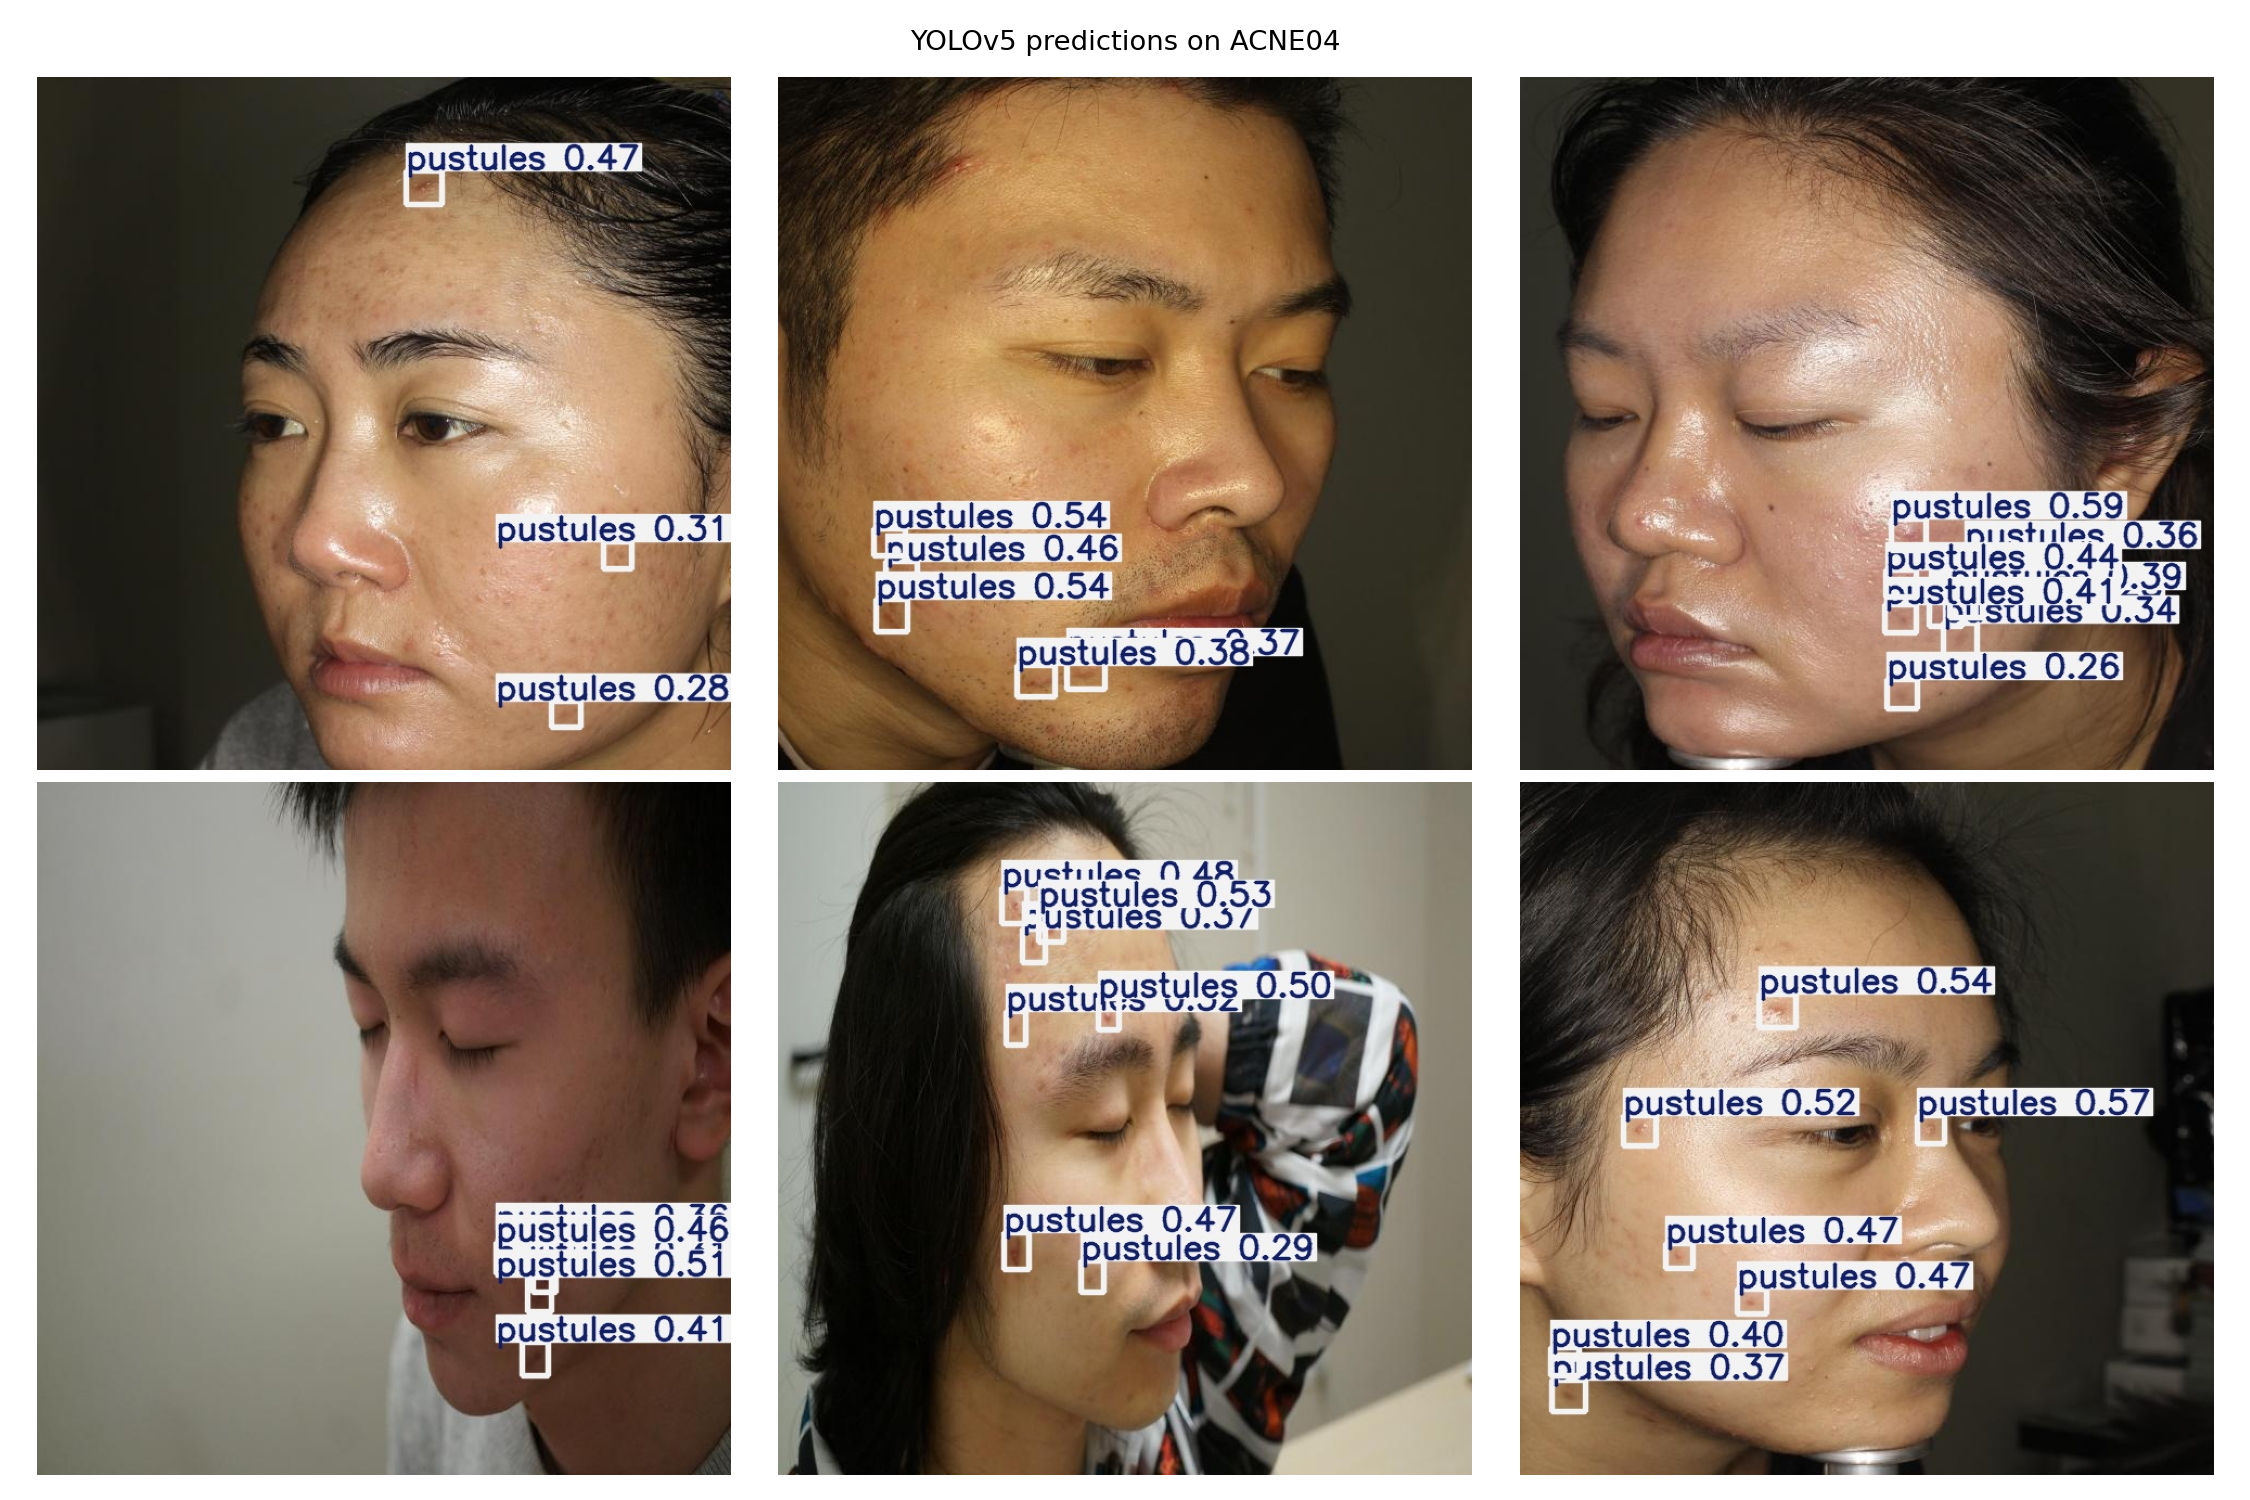
\includegraphics[width=\linewidth]{figures/yolo_predictions.png}
\caption{YOLOv5}
\label{fig:yolo-preds}
\end{subfigure}\hfill
\begin{subfigure}[t]{0.49\textwidth}
\centering
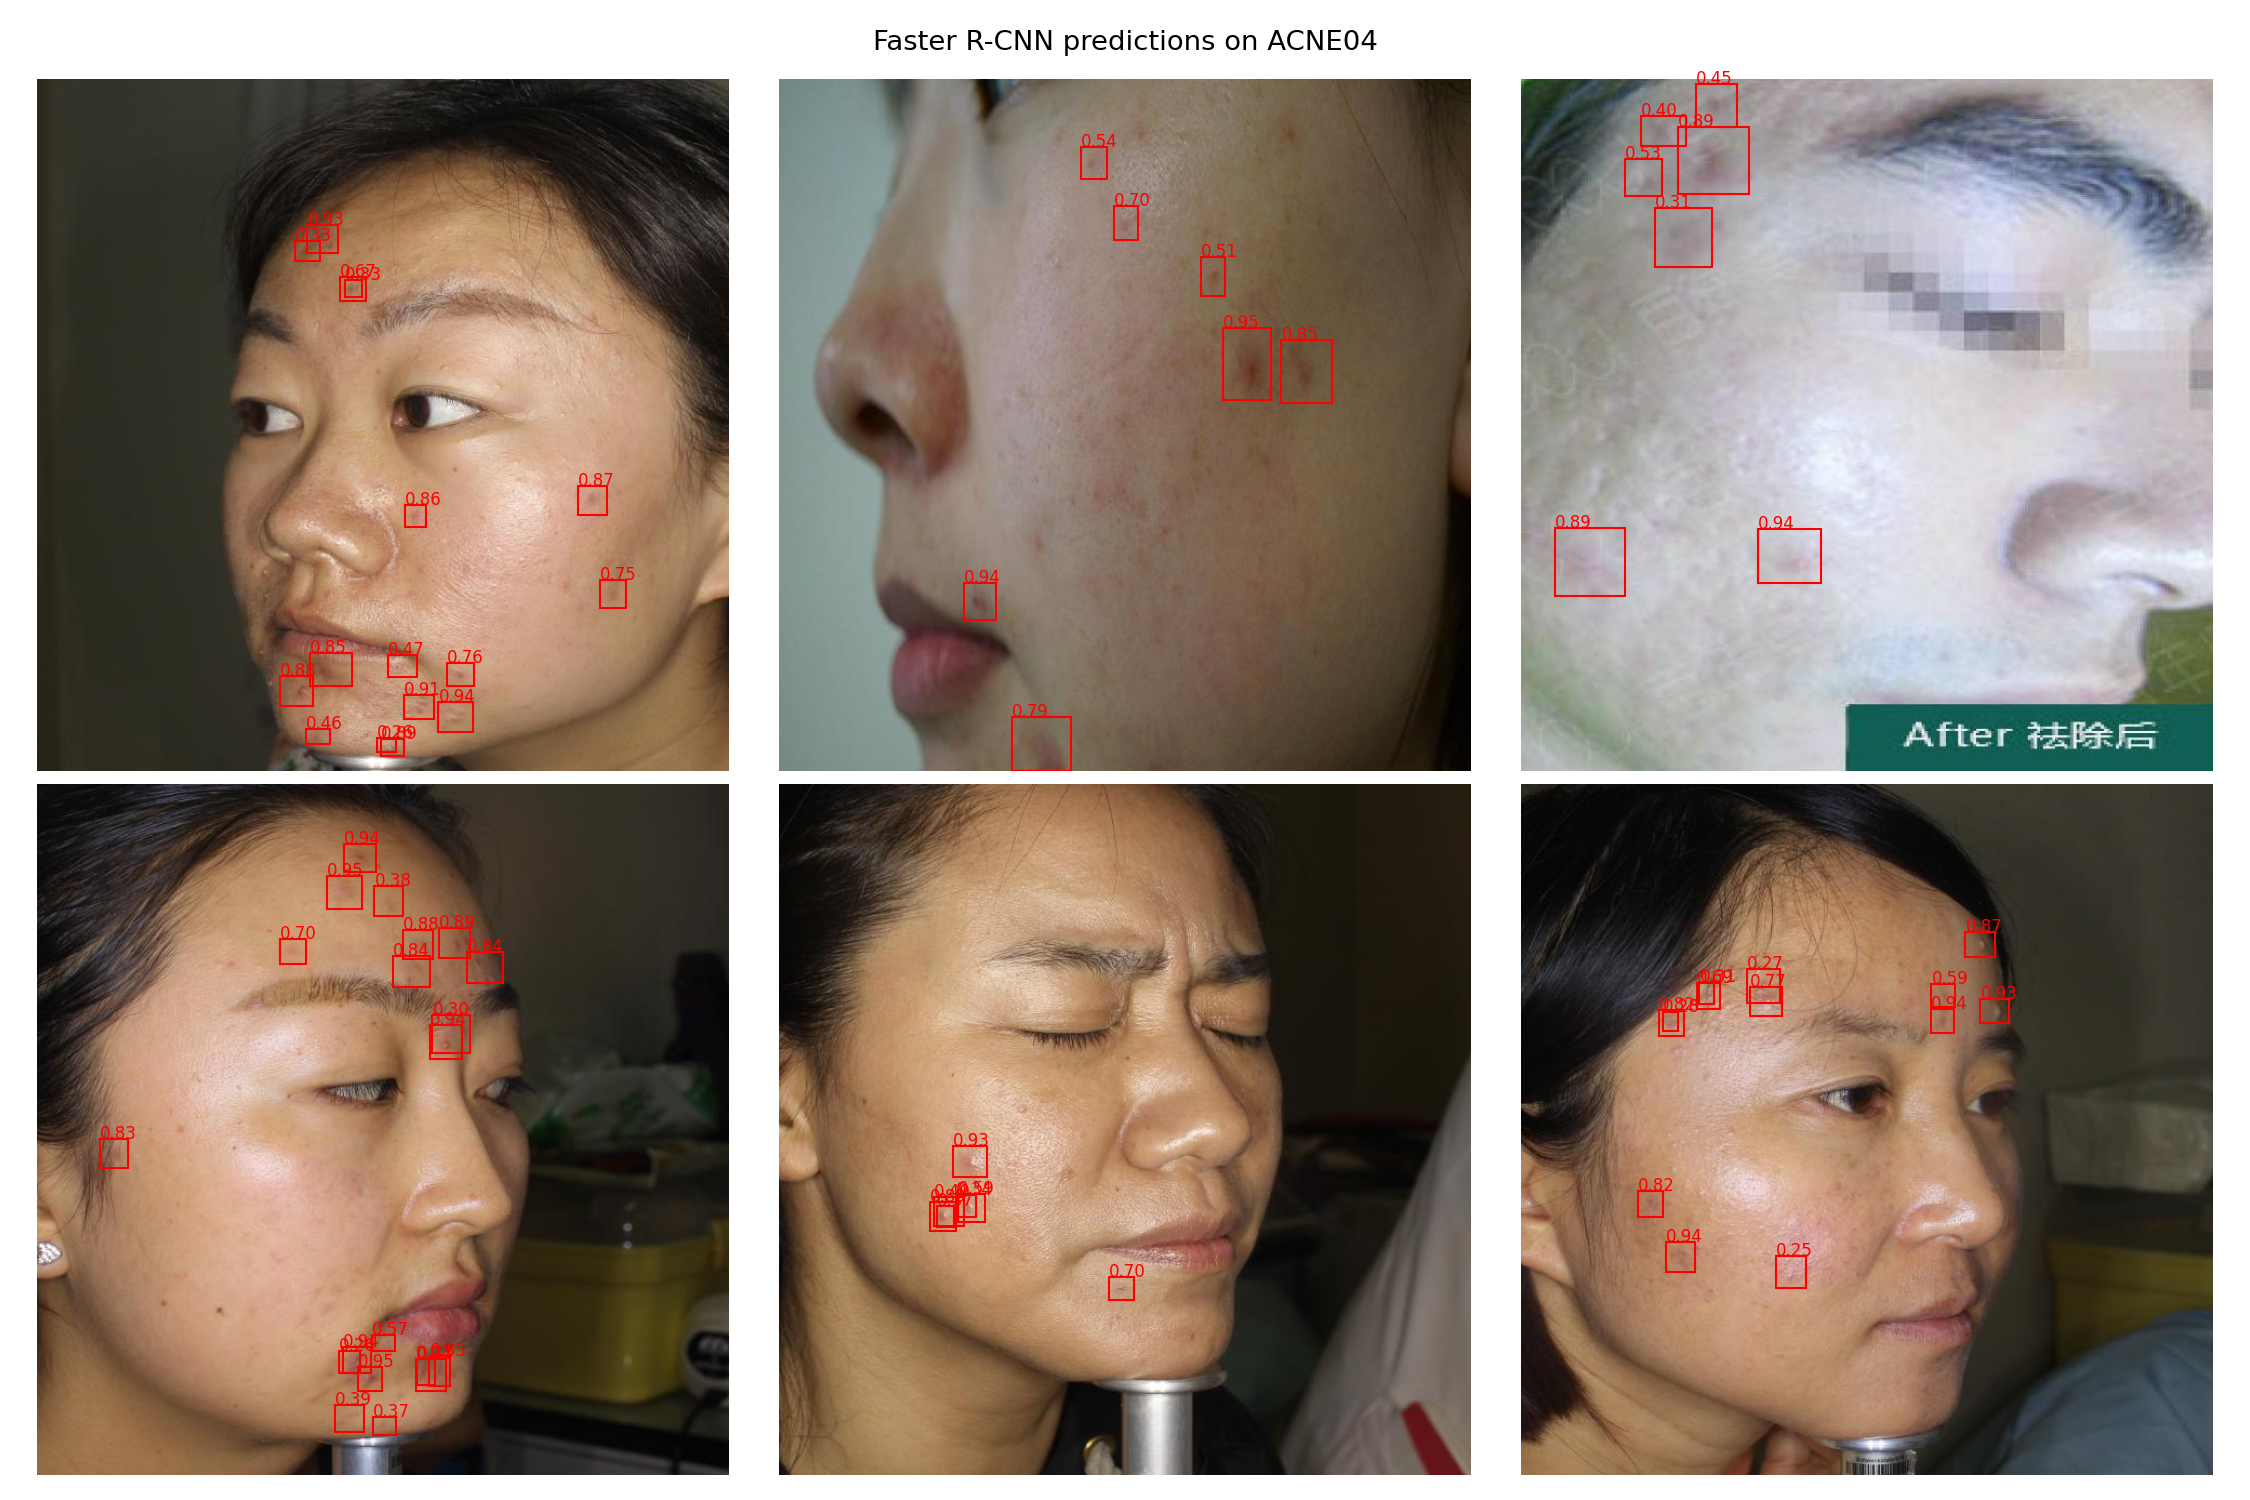
\includegraphics[width=\linewidth]{figures/faster_rcnn_predictions.png}
\caption{Faster R-CNN}
\label{fig:frcnn-preds}
\end{subfigure}
\caption{Qualitative detection on ACNE04 (six test images each).}
\label{fig:det-both}
\end{figure*}

\section{Part 2: Cross-Domain Classification}

\subsection{Patches, baseline, DermNet setup}

Positive/negative $64{\times}64$ patches from ACNE04 boxes (equal counts); box stats checked for scale. \textbf{Baseline:} ResNet-18 ImageNet (He et al., 2016), 10 epochs, Adam $10^{-4}$, flips + color jitter, 80/20 split. DermNet binary: \texttt{Acne and Rosacea Photos} vs.\ all other folders (${\sim}1{:}22$ imbalance). \texttt{ImageFolder} order differs from ACNE04 (\texttt{negative}/\texttt{positive} $\Rightarrow$ acne index 1); evaluation maps label spaces explicitly.

\subsection{Domain adaptation}

(1)~\textbf{\texttt{model\_cls2}:} InceptionResnetV1 VGGFace2 (\texttt{facenet-pytorch}), $160{\times}160$, stronger aug.\ ($45^\circ$ rot., jitter), class weights $[1.0,5.0]$. (2)~\textbf{\texttt{model\_cls3}:} Per-channel histogram matching: each patch is matched to a random reference image from the DermNet \textbf{train} split (acne folder vs.\ pooled non-acne folders), then FaceNet is retrained on the matched patches. (3)~\textbf{\texttt{model\_cls4}:} Pseudo-labels from \texttt{model\_cls3} on \textbf{20 unlabeled DermNet train} images (10 from the acne-related folder + 10 from other folders, shuffled); keep top-$K{=}5$ confident predictions per predicted class; 5 epochs fine-tune at $10^{-5}$.

\subsection{Evaluation}

All checkpoints evaluated with \texttt{evaluate\_on\_dermnet}: resize per model, $P(\text{acne})$, F1-optimal threshold from PR curve; Accuracy, F1 (acne positive), AUROC.

\section{Results}

\begin{table*}[t]
\centering
\scriptsize
\setlength{\tabcolsep}{4pt}
\begin{tabular}{@{}lcc@{}}
\toprule
Metric & YOLOv5 & Faster R-CNN \\
\midrule
mAP@0.5 & \textbf{0.2111} & 0.1945 \\
mAP@0.5:0.95 & \textbf{0.0520} & 0.0413 \\
Precision@0.5 & \textbf{0.3068} & 0.2665 \\
Recall@0.5 & 0.2840 & \textbf{0.4329} \\
Mean IoU@0.5 (matched) & \textbf{0.6323} & 0.6225 \\
\bottomrule
\end{tabular}
\caption{Detection on ACNE04. Faster R-CNN rows are on the COCO \textbf{test} split. YOLO mAP/P/R are from the training run's \textbf{val} split (\texttt{results.csv}); YOLO mean matched IoU@0.5 is on the COCO \textbf{test} split (same images as Faster R-CNN).}
\label{tab:det}
\end{table*}

Table~\ref{tab:det} summarizes Part~1. mAP@0.5 is similar across detectors (${\sim}0.19$--$0.21$) but is \textit{not} measured on identical splits for YOLO vs.\ Faster R-CNN (see caption). On the shared test images, mean matched IoU@0.5 is nearly tied. Faster R-CNN shows higher \textbf{test} recall under the greedy matcher (0.43 vs.\ 0.28 for YOLO's val recall), but the val/test asymmetry means that gap is only directional, not definitive.

\begin{table*}[t]
\centering
\scriptsize
\setlength{\tabcolsep}{3pt}
\begin{tabular}{@{}lcccc@{}}
\toprule
Model & Acc. & F1 & AUROC & Thr. \\
\midrule
Baseline (ResNet-18) & 0.6970 & 0.1918 & 0.6169 & 0.4960 \\
FaceNet + Aug. & \textbf{0.7714} & 0.1759 & 0.5883 & 0.9252 \\
Aug + Hist.\ match & 0.6213 & \textbf{0.1938} & \textbf{0.6340} & 0.1296 \\
Aug + HM + Pseudo & 0.6123 & 0.1901 & 0.6174 & 0.3105 \\
\bottomrule
\end{tabular}
\caption{DermNet binary test (acne vs.\ non-acne), one Colab run (single seed).}
\label{tab:cls}
\end{table*}

Table~\ref{tab:cls} reports Part~2 on the full DermNet binary test set (accuracy, F1, AUROC, and F1-optimal threshold from the PR sweep in \texttt{evaluate\_on\_dermnet}).

\subsection{Grad-CAM}

Grad-CAM on \texttt{model\_cls2}--\texttt{model\_cls4}: 10 DermNet test images each (5 acne / 5 non-acne), FaceNet \texttt{block8}, acne class. Figure~\ref{fig:gradcam-all}: $2{\times}5$ panels; \texttt{True}/\texttt{Pred} with confidence; green/red $=$ correct/incorrect; warm colors $=$ high contribution to acne activation.

\begin{figure*}[t]
\centering
\begin{subfigure}[t]{0.325\textwidth}
\centering
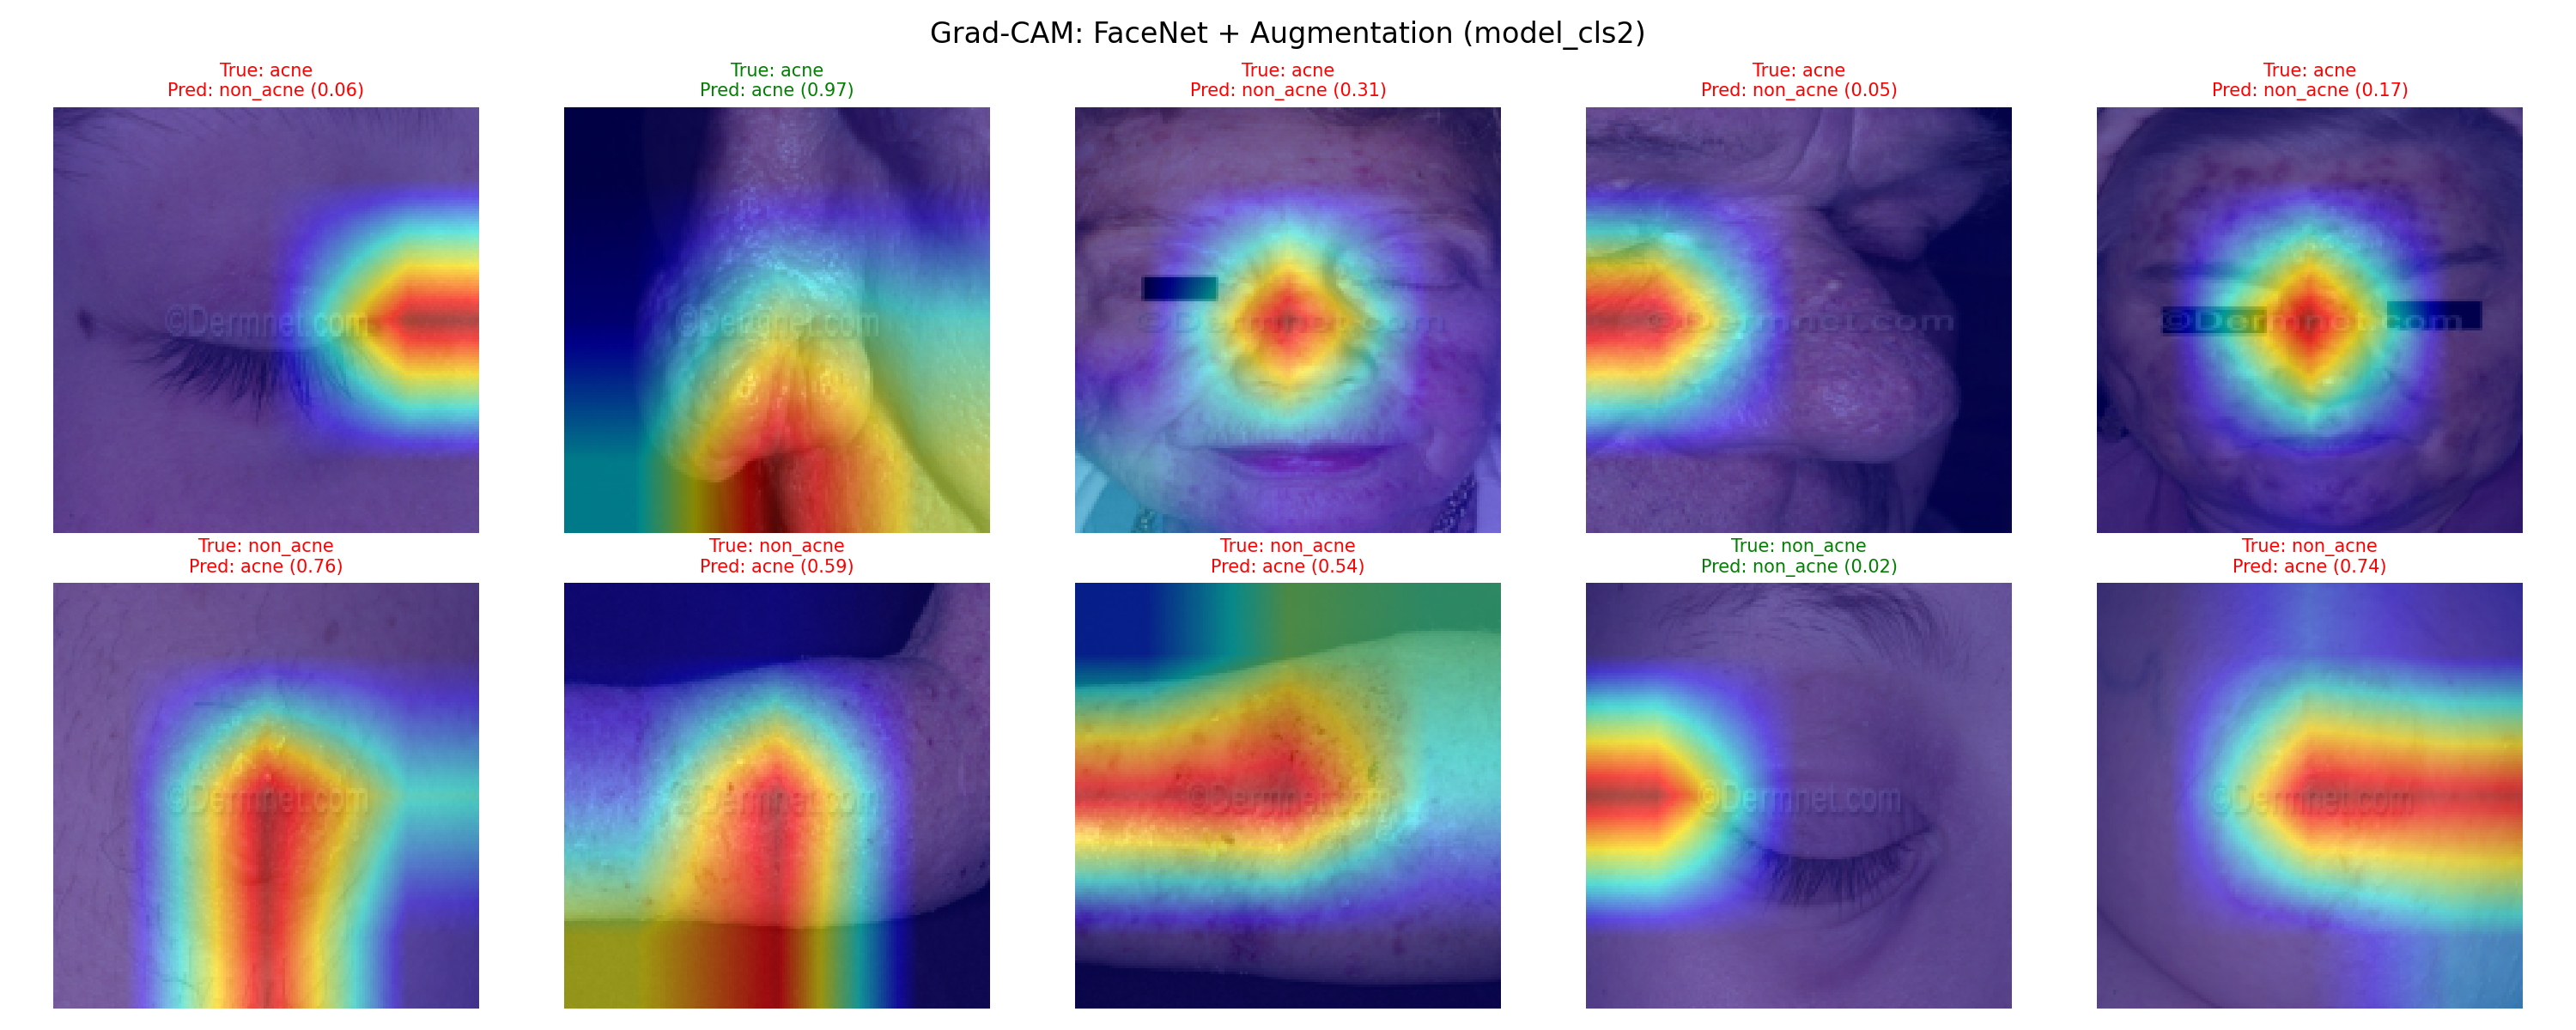
\includegraphics[width=\linewidth]{figures/gradcam_dermnet_cls2.png}
\caption{\texttt{cls2}}
\label{fig:gradcam-cls2}
\end{subfigure}\hfill
\begin{subfigure}[t]{0.325\textwidth}
\centering
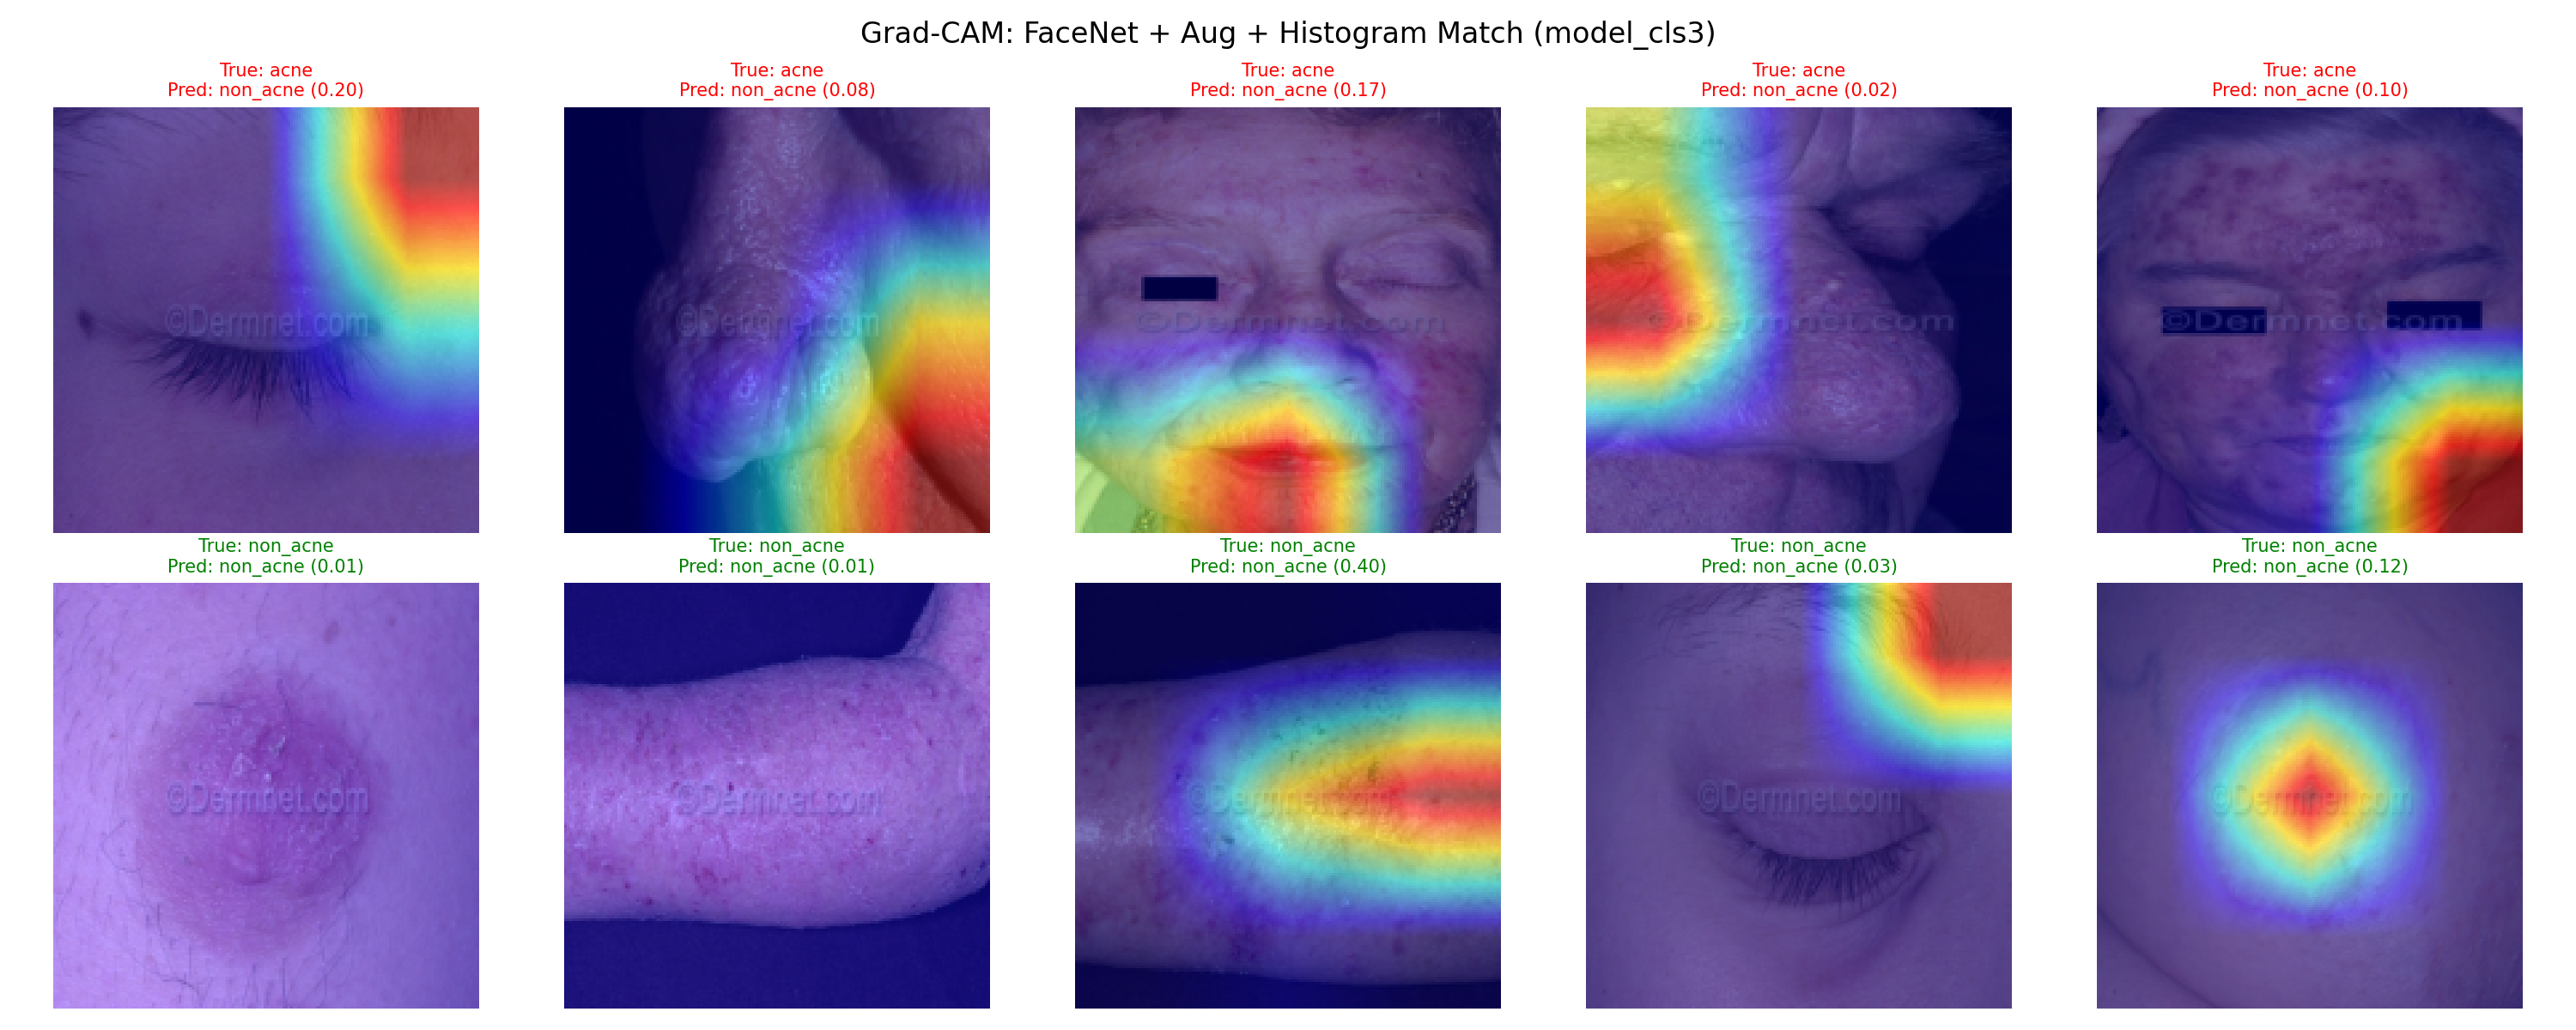
\includegraphics[width=\linewidth]{figures/gradcam_dermnet_cls3.png}
\caption{\texttt{cls3}}
\label{fig:gradcam-cls3}
\end{subfigure}\hfill
\begin{subfigure}[t]{0.325\textwidth}
\centering
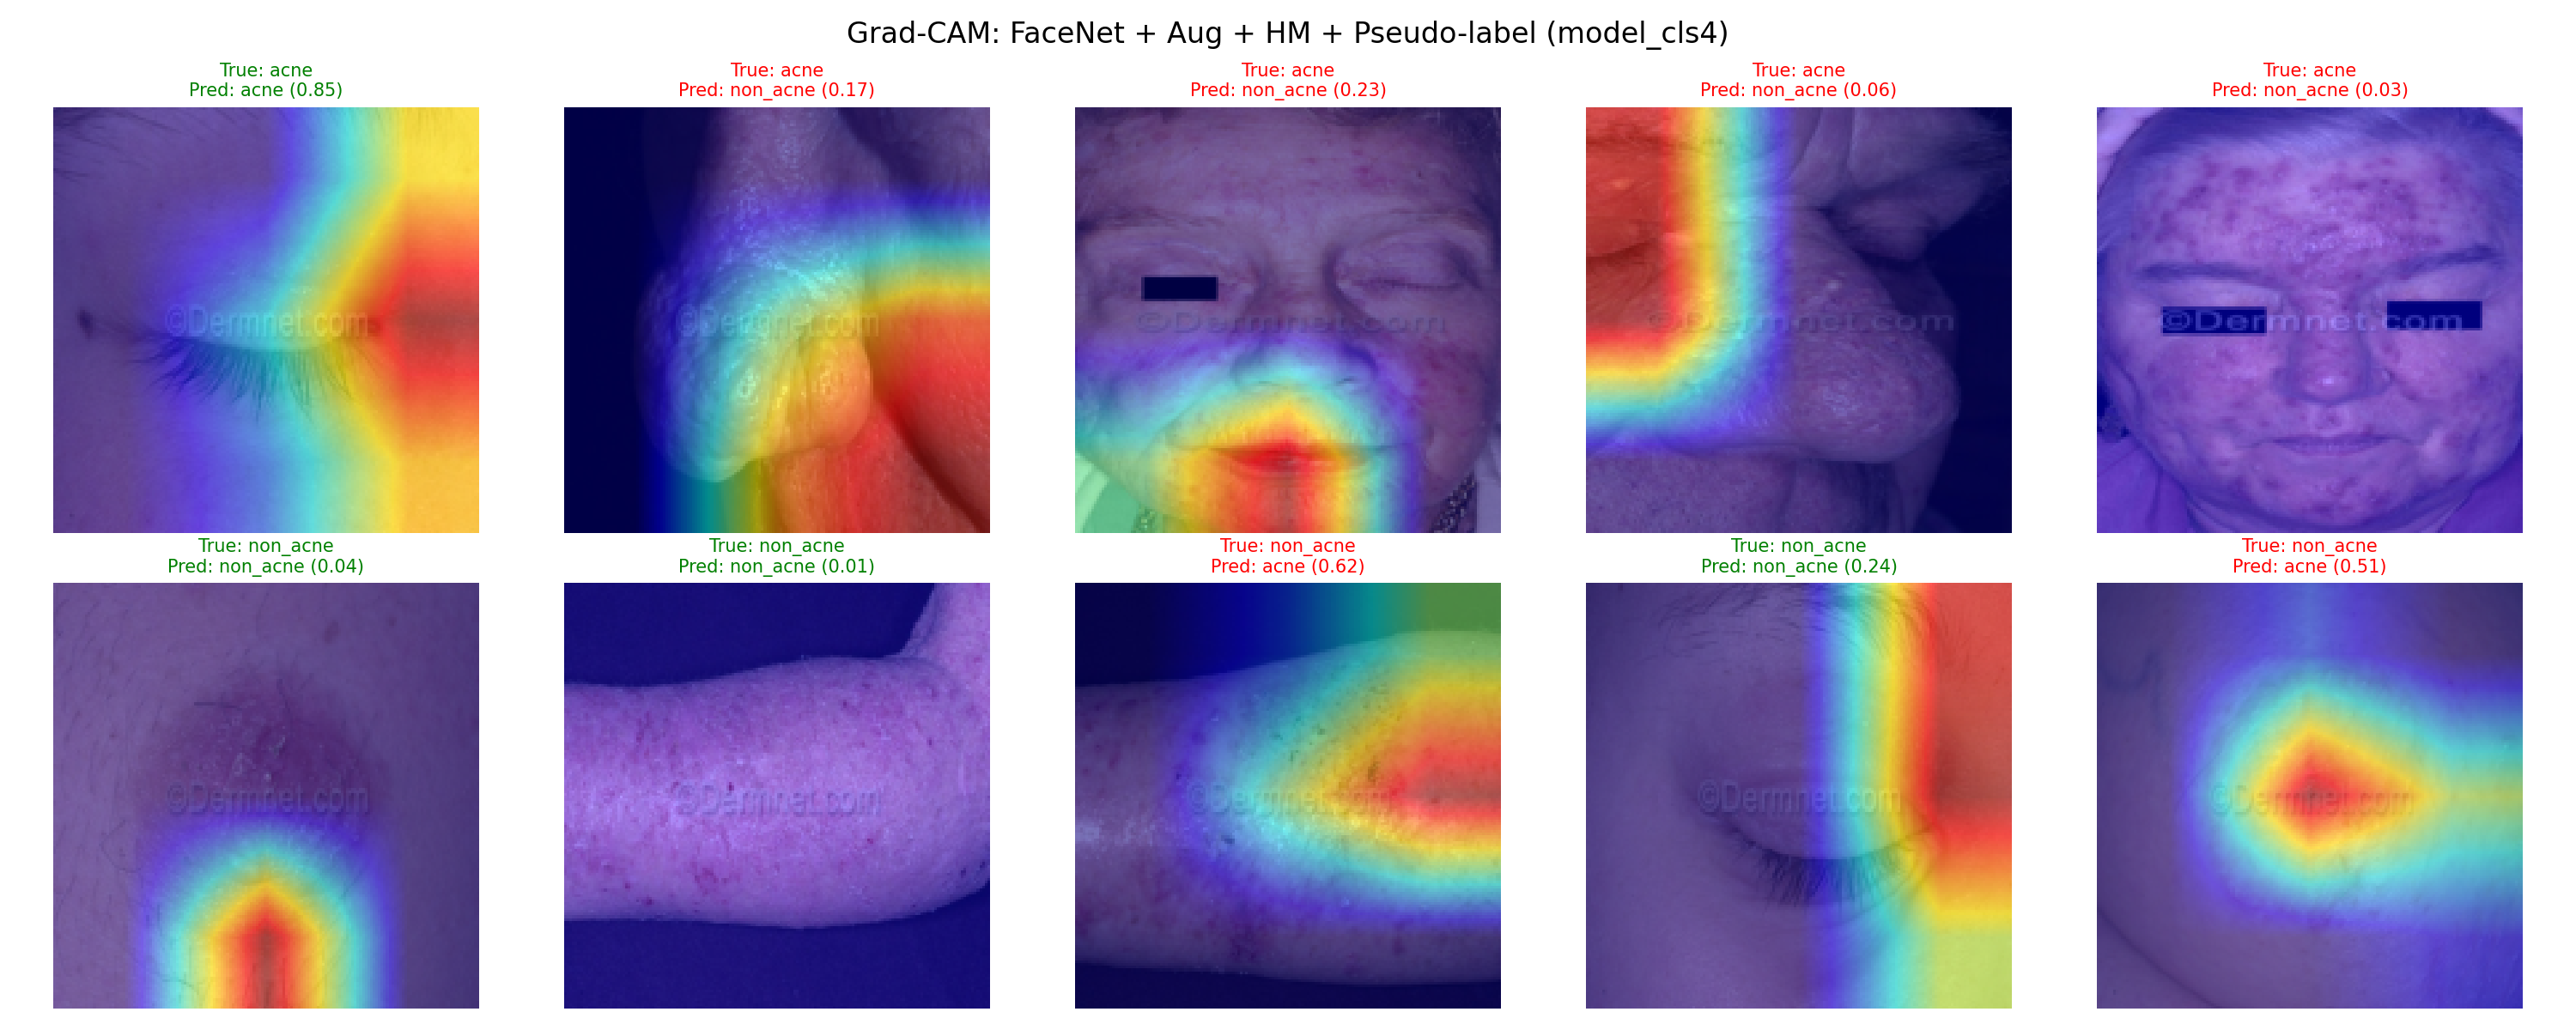
\includegraphics[width=\linewidth]{figures/gradcam_dermnet_cls4.png}
\caption{\texttt{cls4}}
\label{fig:gradcam-cls4}
\end{subfigure}
\caption{Grad-CAM on DermNet (FaceNet \texttt{block8}, acne class).}
\label{fig:gradcam-all}
\end{figure*}

\section{Analysis (reflection)}

\textbf{Transfer headline.} AUROC stays in a narrow band (roughly $0.59$--$0.63$). Histogram matching is best in this run (0.6340), only about $+0.017$ over the baseline (0.6169), so I treat the gain as suggestive rather than conclusive at single-seed.

\textbf{Accuracy vs.\ AUROC.} The augmentation-only checkpoint has the highest accuracy (0.7714) but the worst AUROC (0.5883) and an extreme threshold (0.9252), indicating a conservative operating point on the majority class rather than better acne discrimination. F1 remains low and tightly clustered (${ \sim }0.19$) across all checkpoints.

\textbf{Grad-CAM / failure modes.} Across 30 panels (10 images $\times$ three FaceNet checkpoints), attention repeatedly overlaps the \textbf{DermNet.com watermark}. The shortcut persists after histogram matching and pseudo-labeling, which helps explain why adaptation did not produce a robust AUROC gain: all runs can exploit the same artifact. Low F1 (${\sim}0.19$) across conditions reflects imbalance plus the patch$\to$full-image gap.

\textbf{Next steps.} Inpaint or remove watermarks; report PR-AUC; balanced sampling or focal loss; DANN/CORAL on features; multi-seed runs before claiming method rank order.

\section*{References}
{\footnotesize
\begin{enumerate}[leftmargin=*, itemsep=0pt, topsep=2pt]
\item Ren et al.\ (2015). Faster R-CNN. \url{https://arxiv.org/abs/1506.01497}
\item Redmon \& Farhadi (2018). YOLOv3. \url{https://arxiv.org/abs/1804.02767}
\item Lin et al.\ (2014). MS COCO. \url{https://arxiv.org/abs/1405.0312}
\item He et al.\ (2016). ResNet. \url{https://arxiv.org/abs/1512.03385}
\item Selvaraju et al.\ (2017). Grad-CAM. \url{https://arxiv.org/abs/1610.02391}
\end{enumerate}
}

\end{document}
